../cictikz/src/cictikz/data/tex/cictikz_preamble.tex

% Gate tunneling: the oxide is 1-2 nm thin, so the electron wave
% function is non-zero on the far side. Blue: a channel electron leaking
% into the gate. Red: a gate carrier leaking into the channel.

\definecolor{echarge}{RGB}{30,60,220}
\definecolor{hcharge}{RGB}{220,30,30}

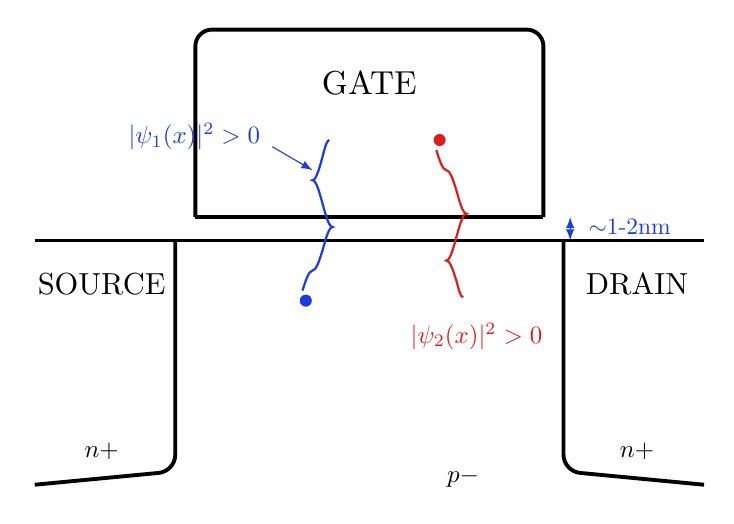
\begin{tikzpicture}[scale=0.85]

  % gate block
  \draw[line width=1.4pt, rounded corners=6pt] (2.4,4.4) -- (2.4,7.2) -- (7.6,7.2) -- (7.6,4.4);
  \node[anchor=center, scale=1.2] at (5.0,6.4) {GATE};

  % thin oxide between gate bottom and the surface
  \draw[line width=1.2pt] (2.4,4.4) -- (7.6,4.4);
  \draw[line width=1.2pt] (0.0,4.05) -- (10.0,4.05);
  \draw[latex-latex, thin, echarge] (8.0,4.4) -- (8.0,4.05);
  \node[echarge, anchor=west, scale=0.85] at (8.15,4.25) {$\sim$1-2nm};

  % source and drain wells
  \draw[line width=1.4pt, rounded corners=6pt] (2.1,4.05) -- (2.1,0.6) -- (0.0,0.4);
  \draw[line width=1.4pt, rounded corners=6pt] (7.9,4.05) -- (7.9,0.6) -- (10.0,0.4);
  \node[anchor=center, scale=1.1] at (1.0,3.4) {SOURCE};
  \node[anchor=center, scale=1.1] at (9.0,3.4) {DRAIN};
  \node[anchor=center, scale=0.9] at (1.0,0.9) {$n+$};
  \node[anchor=center, scale=0.9] at (9.0,0.9) {$n+$};
  \node[anchor=center, scale=0.9] at (6.4,0.5) {$p-$};

  % electron wave function reaching from the channel into the gate
  \draw[echarge, thick]
    (4.0,3.3) sin (4.15,3.6) cos (4.3,3.9) sin (4.45,4.25) cos (4.3,4.6)
    sin (4.15,4.95) cos (4.3,5.3) sin (4.4,5.55);
  \fill[echarge] (4.05,3.15) circle (0.09);
  \node[echarge, anchor=east, scale=0.9] at (3.5,5.6) {$|\psi_1(x)|^2 > 0$};
  \draw[echarge, thin, -latex] (3.55,5.45) -- (4.15,5.1);

  % gate carrier wave function reaching down into the channel
  \draw[hcharge, thick]
    (6.0,5.4) sin (6.15,5.1) cos (6.3,4.8) sin (6.45,4.45) cos (6.3,4.1)
    sin (6.15,3.75) cos (6.3,3.45) sin (6.4,3.2);
  \fill[hcharge] (6.05,5.55) circle (0.09);
  \node[hcharge, anchor=north, scale=0.9] at (6.6,2.95) {$|\psi_2(x)|^2 > 0$};

\end{tikzpicture}
\end{document}
